\section{Szeregowe zapytania dla zbioru FWB\_0}

\begin{figure}[!hb]
	\centering 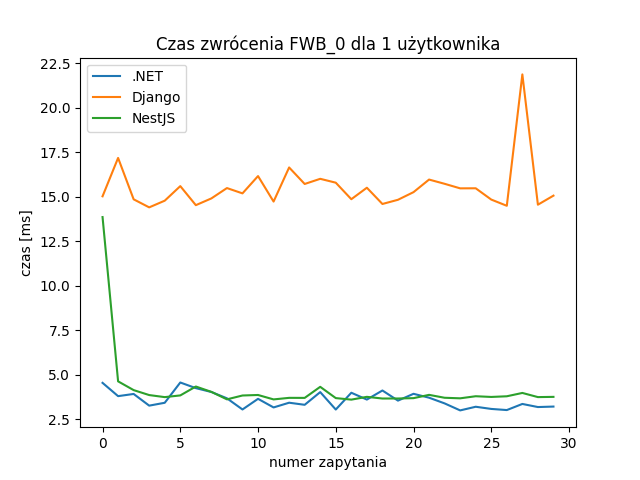
\includegraphics[width=1\linewidth]{rysunki/Czas_zwrocenia_FWB_0_dla_1_uzytkownika.png}
	\caption{Czas zwrócenia zbioru FWB\_0 dla 1 użytkownika}
	\label{rys:request_duration_for_FWB_0}
\end{figure}

Zmierzone wartości otrzymane podczas badania zostały zobrazowane na rysunku \ref{rys:request_duration_for_FWB_0}.
Prezentuje on czas zwrócenia wartości przez framework w mierzonym oknie czasowym.
Standardowe odchylenie dla czasu zmierzononego dla frameworka .NET wyniosło 0,45 ms.
Było to najmniejsze wahanie na tle innych badanych narzędzi.
Dla Django standardowe odchylenie to 1,37 ms.
Trochę większe odchylenie uzyskał NestJS uzyskując wartość 1,84 ms.
Widoczne jest większe odchylenie podczas pierwszego zapytania dla NestJS.
Późniejsze zapytania dostają odpowiedź zdecydowanie szybciej.

\begin{figure}[!hb]
	\centering 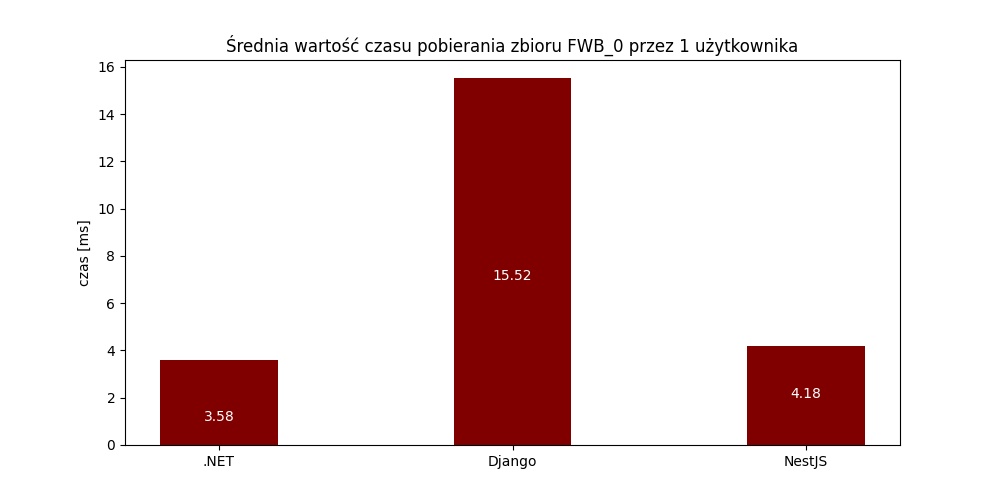
\includegraphics[width=1\linewidth]{rysunki/Srednia_wartosc_czasu_pobierania_zbioru_FWB_0_przez_1_uzytkownika.png}
	\caption{Średni czas zwrócenia zbioru FWB\_0 dla 1 użytkownika}
	\label{rys:mean_duration_for_FWB_0}
\end{figure}

Średni czas zwrócenia odpowiedzi podczas tego badania został zaprezentowany na rysunku \ref{rys:mean_duration_for_FWB_0}.
Zdycydowanie najdłuższy odpowiedzi przypadł Django osiągając wynik 15,52 ms.
Około 3 razy mniejszy czas uzyskał NestJS.
Wygranym tego zestawienia został .NET uzyskując najszybszy średni czas odpowiedzi na poziomie 3.58 ms.
